%%%
% set up document type
%%%
\documentclass[12pt]{article}

%%%
% declare all packages
%%%
\usepackage[left=25mm, top=20mm, right=25mm, bottom=30mm,nohead,nofoot]{geometry} 

\usepackage[T2A]{fontenc}
\usepackage[utf8]{inputenc}
\usepackage[english, russian]{babel}

\usepackage{graphics, graphicx}

\usepackage{url}
\usepackage{hyperref}

\usepackage{amssymb,latexsym} 
\usepackage{MnSymbol}
\usepackage{mathrsfs}

\usepackage[nottoc,numbib]{tocbibind}
\usepackage{float}
\usepackage{listings}
\usepackage{multirow}
\usepackage{hhline}
\usepackage{delarray}

\usepackage{color,colortbl}

% \usepackage{verbatim}
%%%
% document settings
%%%
\setcounter{tocdepth}{4}
\graphicspath{ {./pic/} }

\renewcommand{\listoffigures}{\begingroup  % add number to list of graphics
\tocsection
\tocfile{\listfigurename}{lof}
\endgroup}
\renewcommand{\listoftables}{\begingroup  % add number to list of tables
\tocsection
\tocfile{\listtablename}{lot}
\endgroup}

%******************************************************************
%******************************************************************
\begin{document}

\begin{titlepage}
	\center
		Санкт-Петербургский Политехнический 
		университет \\ Петра Великого\\
		Институт прикладной математики и механики
		\\ \textbf{Высшая школа прикладной математики и вычислительной физики}

	\vfill ~
	\textbf{
		\\ \large ЛАБОРАТОРНАЯ РАБОТА №3
	}
	\\	на тему 
	\\ "Метод конечных объёмов для уравнений эллиптического типа"
	\\ по дисциплине
	\\ "Конечно-разностные и сеточные методы"

	\vfill ~

	Выполнил студент гр. \textbf{3630102/60101} \\
	\textbf{Лансков.Н.В.} \\ 

\vfill

{\large}	Санкт-Петербург
\\ 2020
\end{titlepage}

%%%
% Table of conetnts 
%%%

\tableofcontents 
\newpage
\listoffigures
\newpage
\listoftables
\newpage

%%%
% Text
%%%
\section{Постановка задачи}

Будем решать задачу:

$$
\begin{cases}
-\dfrac{\partial}{\partial x}\left( a(x,y) \dfrac{\partial u}{\partial x}\right) - \dfrac{\partial}{\partial x}\left( a(x,y) \dfrac{\partial u}{\partial x}\right) + q(x,y)u = f(x,y)
\\ \\
0 < \alpha < a, b < \beta; 0 < q_m < q; & (x,y) \in [3, 3.4] \times [1, 1.4] = \Omega
\\ \\
u|_{\partial \Omega} = g(x, y)
\end{cases}
$$

В данной лабораторной исследуется задача со следующими параметрами:
$$
\begin{cases}
a(x,y) = x + y \\ 
b(x,y) = 1 + xy \\
q(x,y) = x^4 \\
g(x,y) = cos(2x) \cdot e^{-3y} \\
f(x,y) = 3xcos(2x)e^{-3y}+4xsin(2x)e^{-3y} - 9cos(2x)e^{-3y}(xy + 1) + x^4cos(2x)e^{-2y} + \\ + 4cos(2x)e^{-3y}(x^2 + y^2)
\end{cases}
$$

\section{Метод конечных объёмов}

Рассмотрим  процесс нахождения коэффициентов по методу конечных объёмов.

Разобъём нашу область на конечные объёмы (с центрами во внутренних в узлах сетки). Тогда для каждой внутреней точки рассматриваем конечный объём $\Omega_{ij}$. Далее приведём вычисления в общем виде для такого конечного объёма.

Проинтегрируем уравнение 1 по конечному объёму и домножим на -1:
\begin{equation}
\int\limits_{\Omega_{ij}}{\left[ \dfrac{\partial}{\partial x}\left( a\dfrac{\partial u}{\partial x}\right) + \dfrac{\partial}{\partial y}\left( b\dfrac{\partial u}{\partial y}\right) \right]d\Omega}
 - \int\limits_{\Omega_{ij}}qud\Omega = \int\limits_{\Omega_{ij}}fd\Omega 
\end{equation}

Подробнее рассмотрим первое слагаемое из левой части. Под интегралом стоит дивергенция, применяем формулу Остроградского-Гаусса, получаем следующее выражение:

\begin{eqnarray}
\oint\limits_{\gamma_{ij}}{\left[ a\dfrac{\partial u}{\partial x}cos(n,x) + b\dfrac{\partial u}{\partial y}cos(n,y) \right]d\gamma} = \left[ \omega^x = a\dfrac{\partial u}{\partial x}; \omega^y =  b\dfrac{\partial u}{\partial y} \right] = 
\\
 = \left( w_{i+0.5,j}^x - w_{i-0.5,j}^x \right) h_y + 
\left( w_{i,j+0.5}^y - w_{i,j-0.5}^y \right) h_x 
\end{eqnarray}

Тут мы произвели определённую замену переменных и раскрыли косинусы, появившиеся после применения формулы О-Г. С учётом данной замены, легко видеть, что выполнены следующие равенства:

\begin{equation}\label{eq1}
\int\limits_{\Omega_{ij}^{'}}{\dfrac{\omega^x}{a}d\Omega} = \int\limits_{\Omega_{ij}^{'}}{\dfrac{\partial u}{\partial x}d\Omega} 
\end{equation}
\begin{equation}\label{eq2}
\int\limits_{\Omega_{ij}^{''}}{\dfrac{\omega^y}{b}d\Omega} = \int\limits_{\Omega_{ij}^{''}}{\dfrac{\partial u}{\partial y}d\Omega}
\end{equation}

Рассмотрим подробнее (\ref{eq1}). Применяя к правой части теорему О-Г., а левую часть преобразовав определённым образом, получаем уже конечно-разностное выражение.

$$
(\ref{eq1}) \Longleftrightarrow \omega_{i+0.5,j}^x \cdot \int\limits_{\Omega_{ij}^{'}}{\dfrac{d\Omega}{a}} = (v_{i+1,j} - v_{ij})h_y
$$

Отсюда легко можно найти выражение для $\omega_{i+0.5,j}^x$, посчитав численно интеграл. Точно также рассматриваем (\ref{eq2}), и сразу записываем итоговое выражение, сгруппировав слагаемые при соответствующих узновых точках.

\begin{eqnarray}
\left( \dfrac{p_{i+0.5, j} + p_{i-0.5, j}}{h_x^2} + \dfrac{q_{i, j+0.5} + q_{i, j-0.5}}{h_y^2} + \dfrac{\rho_{ij}}{h_xh_y} \right) v_{ij} - \nonumber \\
\left( \dfrac{p_{i-0.5, j}v_{i-1,j} + p_{i+0.5, j}v_{i+1,j}}{h_x^2} + \dfrac{q_{i, j+0.5}v_{i,j+1} + q_{i, j-0.5}v_{i,j-1}}{h_y^2} \right) = g_{ij}
\end{eqnarray}

Все вышеперечисленные выражения я привёл в общем виде для упрощения восприятия. Теперь рассмотрим, чему равны коэффициенты в контексте конкретной задачи.

\begin{equation}
\begin{cases}
p_{i+0.5,j} = \int\limits_{\Omega_{ij}^{'}}{\dfrac{d\Omega}{x + y}} &
p_{i-0.5,j} = \int\limits_{\Omega_{i-1,j}^{'}}{\dfrac{d\Omega}{x + y}} \\
q_{i,j+0.5} = \int\limits_{\Omega_{ij}^{''}}{\dfrac{d\Omega}{1 + xy}} &
q_{i,j-0.5} = \int\limits_{\Omega_{i,j-1}^{''}}{\dfrac{d\Omega}{1 + xy}} \\
\rho_{ij} = \int\limits_{\Omega_{ij}}{x^4 d \Omega} \\
g_{ij} = \int\limits_{\Omega_{ij}}{fd \Omega} 
\end{cases}
\end{equation}

Замечание о численном вычислении интегралов. Я вычисляю интегралы по следующей формуле (Формула Гаусса для двумерного случая):

\begin{equation}
\int\limits_{[x_0; x_1] \times [y_0; y_1]}{\phi(x, y)d\Omega} = \dfrac{(x_1-x_0)(y_1-y_0)}{4} \sum\limits_{i=1}^4\phi\left(x_0 + \dfrac{(\xi_i+1)(x_1-x_0)}{2} ,y0 + \dfrac{(\eta_i+1)(y_1-y_0)}{2} \right)
\end{equation}
Где $\xi_i$ и $\eta_i$ представляют все пары вида $\left(\dfrac{\pm 1}{\sqrt{3}}; \dfrac{\pm 1}{\sqrt{3}}\right)$
 
\section{Метод Якоби}

Будем применять итерационную процедуру метода Якоби в следующем виде:

\begin{equation}
v_{i,j}^{k+1} = \dfrac{1}{A_{i,j}} \cdot (G_{i,j} - D_{i,j}v_{i-1,j}^{k} - C_{i,j}v_{i,j-1}^{k} - E_{i,j}v_{i,j+1}^{k} - B_{i,j}v_{i+1,j}^{k})
\end{equation}

\section{Метод Зейделя}

Будем применять итерационную процедуру метода Зейделя в следующем виде:

\begin{equation}
v_{i,j}^{k+1} = \dfrac{1}{A_{i,j}} \cdot (G_{i,j} - D_{i,j}v_{i-1,j}^{k+1} - C_{i,j}v_{i,j-1}^{k+1} - E_{i,j}v_{i,j+1}^{k} - B_{i,j}v_{i+1,j}^{k})
\end{equation}

Заметим, что соответствующие значения $v$ при коэффициентах $C$ и $D$ на момент расчёта $v_{i,j}$ уже известны.

\section{Метод SOR}

Будем применять итерационную процедуру метода SOR в следующем виде:

\begin{equation}
v_{SOR}^{k+1} = v_{SOR}^{k} + \omega (v_{Z}^{k+1} - v_{SOR}^{k})
\end{equation}

Где $v_{Z}$ - вычисляется по методу Зейделя

\section{Результаты}
\subsection{Метод Якоби}

Для достижения точности $\varepsilon = 10^{-3}$ возьмём чило разбиений равным $N = 100$ и $\varepsilon_{iter} = \dfrac{10^{-4}\pi^2}{2N^2}$. 

\begin{figure}[H]
\centerline{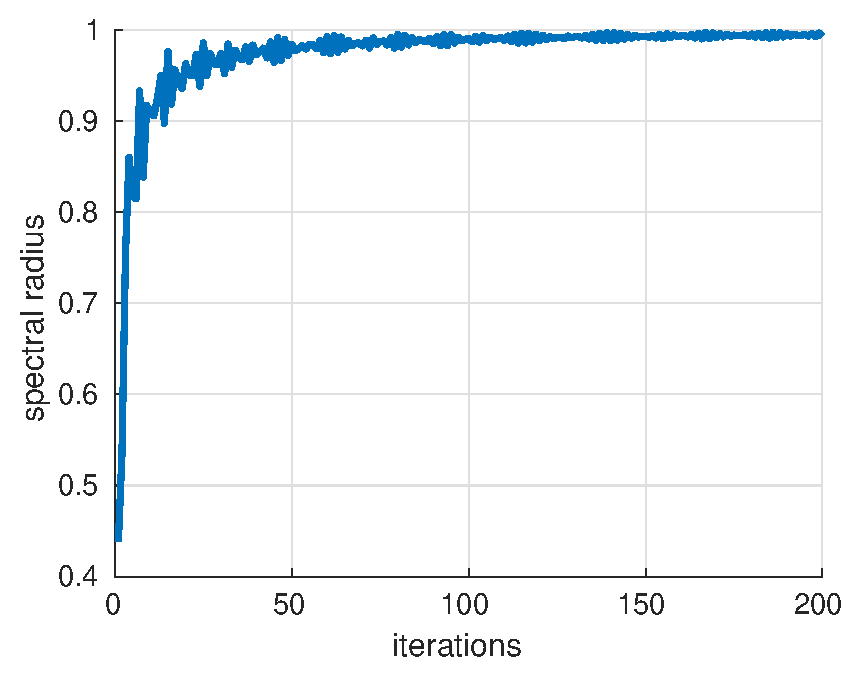
\includegraphics[scale = 0.8]{jacobiSpectre.eps}}
\caption{Зависимость спектрального радиуса от числа итераций}
\end{figure} 

При этом $\rho_{J} = \lim\limits_{k\rightarrow \inf}{\dfrac{||v^{k+1} - v^{k}||}{||v^{k} - v^{k-1}||}} = 0.99945 \approx 0.99950 $, что согласуется с теоретическим значением.
 
\subsection{Метод Зейделя}

Для достижения точности $\varepsilon = 10^{-3}$ возьмём чило разбиений равным $N = 100$ и $\varepsilon_{iter} = \dfrac{10^{-4}\pi^2}{N^2}$. 

\begin{figure}[H]
\centerline{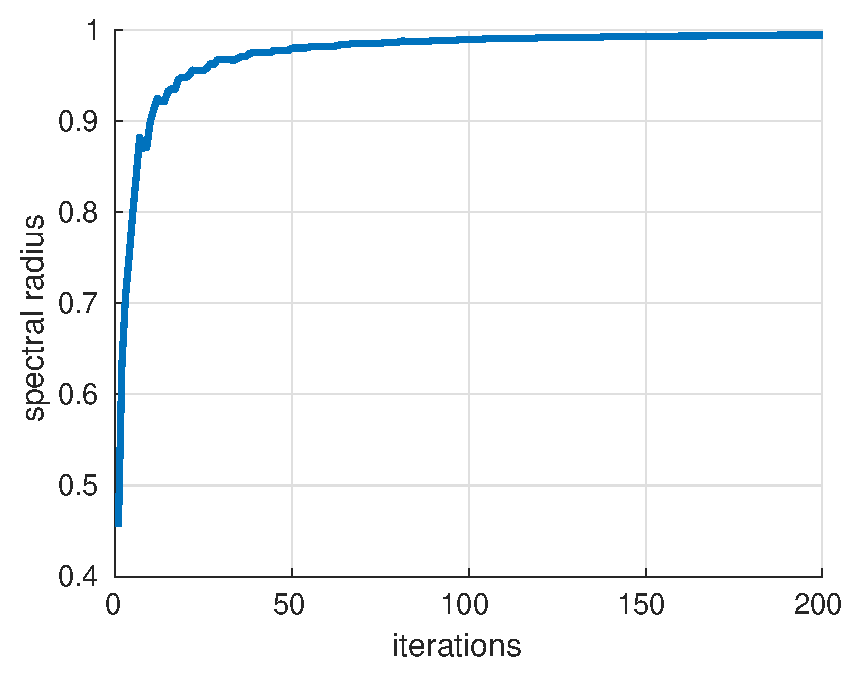
\includegraphics[scale = 0.8]{zeidelSpectre.eps}}
\caption{Зависимость спектрального радиуса от числа итераций}
\end{figure} 

При этом $\rho_{Z} = \lim\limits_{k\rightarrow \inf}{\dfrac{||v^{k+1} - v^{k}||}{||v^{k} - v^{k-1}||}} = 0.99855 \approx 0.9990 = \rho_{J}^2$, что согласуется с теоретическим значением.

\subsection{Метод SOR}

Для достижения точности $\varepsilon = 10^{-3}$ возьмём чило разбиений равным $N = 100$ и $\varepsilon_{iter} = \dfrac{10^{-7}\pi}{N}$.

\begin{figure}[H]
\centerline{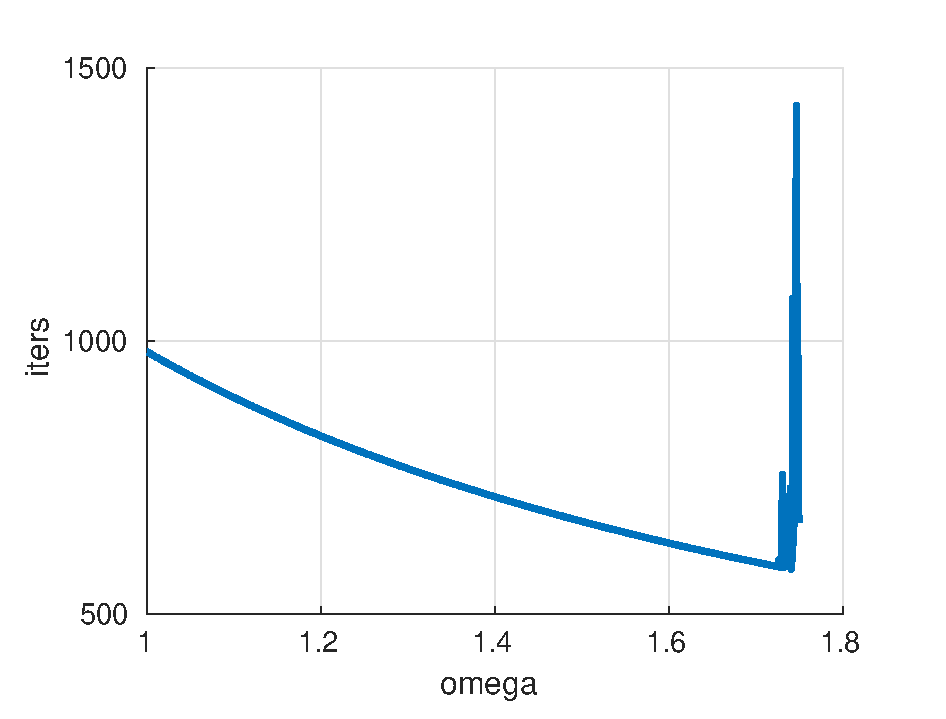
\includegraphics[scale = 0.8]{sor.eps}}
\caption{Зависимость числа итераций $n(\varepsilon)$ от параметра релаксации $\omega$}
\end{figure} 

\begin{figure}[H]
\centerline{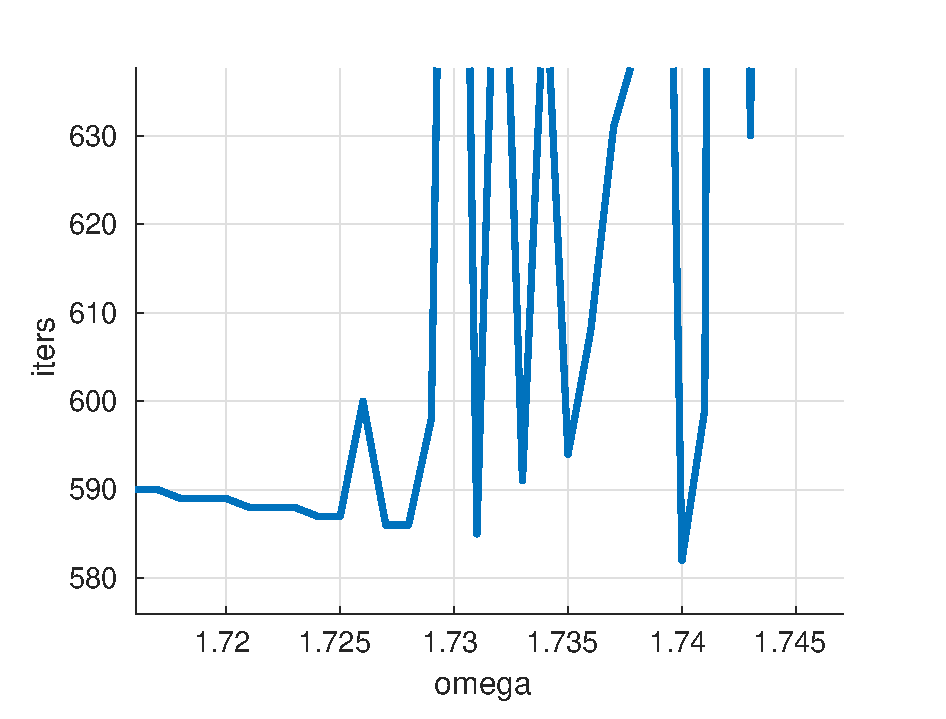
\includegraphics[scale = 0.8]{sor2.eps}}
\caption{Зависимость числа итераций $n(\varepsilon)$ от параметра релаксации $\omega$ (приближение)}
\end{figure} 

По графику видно, что оптимальным параметром релаксации будет $\omega = 1.73$. Однако, из теории следует, что оптимальный параметр должен равняться: $\omega_{opt} = \dfrac{2}{1+\sqrt{1 - \rho_{Z}}} \approx 1.9387$. Я пытался добиться большей точности от графического метода нахождения $\omega_{opt}$ изменяя $N$ и $\varepsilon_{iter}$, но мои попытки не принесли результатов, так как схема начинала терять устойчивость. Я думаю, что всё дело в выбранной мной конкретной задаче, и можно было бы теоретически подобрать исходную задачу точнее, чтобы получить лучший результат. Я же буду далее использовать полученное мною значение $\omega_{opt} = 1.73$.

\subsection{Сравнение методов}

\begin{table}[H]
\caption{Сравнение методов}
\begin{center}
\begin{tabular}{|c|c|c|c|}
\hline
Метод & $\rho$ & $\varepsilon_{iter}$ & $n(\varepsilon)$ \\
\hline
Jacobi & 0.99945 & 4.934802e-08 & 17712 \\
\hline
Zeidel & 0.99855 & 9.869604e-08 & 8858 \\
\hline
SOR & 0.9744 & 1.121997e-08 & 445 \\
\hline
\end{tabular}
\end{center}
\end{table}


\begin{figure}[H]
\centerline{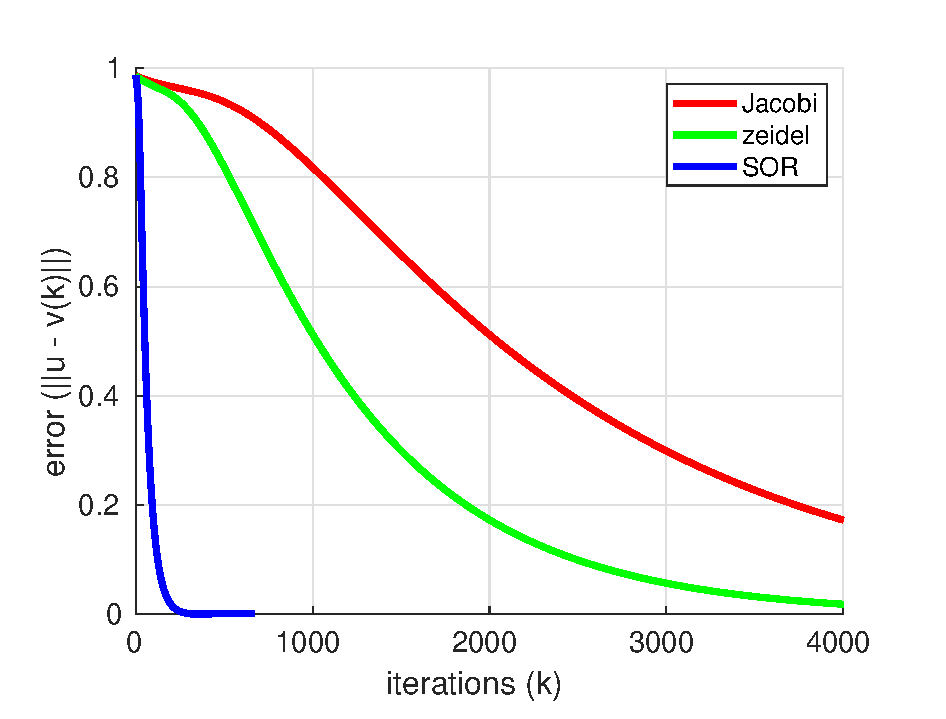
\includegraphics[scale = 0.8]{compare.eps}}
\caption{Сравнение зависимостей $||z^k||$ от числа итераций}
\end{figure}

\newpage

\section{Выводы}

В результате работы были рассмотрены 3 итерационных метода(Якоби, Зейделя, SOR) решения СЛАУ, построенной по МКО. Я получил полное соответствие практичеких и теоретических оценок скоростей сходимости методов, спектральных радиусов и соотношения числа итераций, за исключением $\omega_{opt}$. Как уже выше упоминалось, я считаю что это связано с конкретной задачей.

\section{Приложения}
Исходные файлы лабораторной работы можно найти тут: \\
\url{https://github.com/LanskovNV/numerical/tree/master/net_methods/lab_3}
\end{document}

